\documentclass[11pt]{beamer}
\usetheme{CambridgeUS}
\usepackage[utf8]{inputenc}
\usepackage[spanish]{babel}
\usepackage{amsmath}
\usepackage{amsfonts}
\usepackage{amssymb}
\usepackage{listings}
\usepackage{graphicx}
\usepackage{ragged2e}
\usepackage{adjustbox}
\decimalpoint
\author{Carlos Enrique Ponce Villagran}
\title[Análisis de los equipos de la NFL]{Análisis del Desempeño de los equipos de la NFL en 1976}
%\setbeamercovered{transparent} 
%\setbeamertemplate{navigation symbols}{} 
\logo{
\includegraphics[width=1cm]{../../LogoFCFM-UAS.png} } 
\institute[FCFM]{Facultad de ciencias Físico-Matemáticas} 
\date{11 de diciembre de 2019} 
%\subject{} 

\setbeamercolor{section number projected}{bg=red,fg=white}

\apptocmd{\frame}{}{\justifying}{}

\begin{document}

\begin{frame}
\titlepage
\end{frame}

\begin{frame}{Tabla de Contenido}
\tableofcontents
\end{frame}

\section{Contexto del Problema}

\begin{frame}
\tableofcontents[currentsection]
\end{frame}

\begin{frame}
El modelo se consideran las siguientes regresoras\\
 $x_{1}:=$\textit{Yardas por tierra (temporada)}\\
 $x_{2}:=$\textit{Yardas por aire (temporada)} \\
 $x_{3}:=$\textit{Promedio de pateo (temporada)}\\
 $x_{4}:=$\textit{Porcentaje de goles de campo (GC hechos/GC intentados, temporada)}\\
 $x_{5}:=$\textit{Diferencia de pérdida de balón (pérdidas ganadas/pérdidas perdidas)}\\
$x_{6}:=$\textit{Yardas de castigo (temporada)}  
 $x_{7}:=$\textit{Porcentaje de Carreras (jugadas por tierra/jugadas totales)} \\
  $x_{8}:=$\textit{Yardas por tierra del contrario (temporada)} \\
  $x_{9}:=$\textit{Yardas por aire del contrario (temporada)}\\
  
  y se desea saber si existe una relación con \\
  $Y:=$\textit{Juegos ganados (por temporada de 14 juegos)}
\end{frame}

\begin{frame}
\begin{figure}[hbtp]
\centering
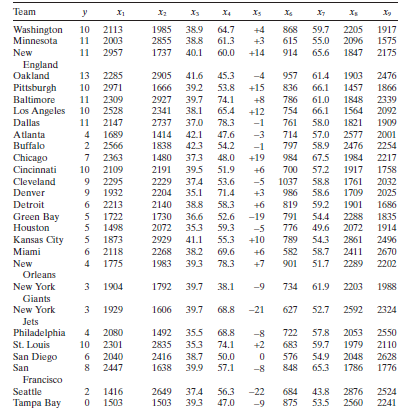
\includegraphics[width=6cm]{TablaDatos.png}
\caption{Datos del Problema}
\end{figure}

\end{frame}

\section{Modelo Inicial}

\subsection{Regresión Lineal Múltiple}

\begin{frame}{}
\tableofcontents[currentsection,currentsubsection]
\end{frame}

\begin{frame}
El modelo inicial estaba constituido por las regresoras:\\


$x_{2}:=$\textit{Yardas por aire (temporada)} \\
$x_{7}:=$\textit{Porcentaje de Carreras (jugadas por tierra/jugadas totales)} \\
$x_{8}:=$\textit{Yardas por tierra del contrario (temporada)}\\


donde la tabla de análisis de varianza arrojo los siguientes resultados.

\end{frame}

\begin{frame}
Primero se procedió a calcular el anova del modelo\\~\\
\begin{adjustbox}{width=1\textwidth}
\begin{tabular}{ccccc}
\hline 
\textbf{Fuente de Variación} & \textbf{Suma de Cuadrados} & \textbf{Grados de Libertad} & \textbf{Cuadrado medio} & $F_{0}$ \\ 
\hline 
Regresión & 257.0671 & 3 & 85.68903 & 29.42231 \\ 
Residuales & 69.8972 & 24 & 2.912383 &  \\ 
Total & 326.9643 & 27 &  &  \\ 
\hline 
\end{tabular} 
\end{adjustbox}\\~\\
donde se concluyo que la hipótesis nula global del modelo se rechaza con $100(1-\alpha)\%$ si $F_{0}>F_{\alpha,3,24}$, por ejemplo a un nivel de significancia $\alpha=0.05$ la hipótesis nula se rechaza.
\end{frame}

\begin{frame}
\begin{itemize}
\justifying
\item[\textcolor{red}{\textbullet}] Además, se obtuvo que cada una de las regresoras ($x_{2}$, $x_{7}$ y $x_{8}$) contribuían de forma significante al modelo haciendo sus respectivas pruebas de hipótesis individuales.

\item[\textcolor{red}{\textbullet}] Por ultimo se procedió a obtener los valores de $R^{2}=0.7862$ y $R^{2}_{Adj}=0.7595$.
\end{itemize}
\end{frame}

\begin{frame}

\begin{itemize}
\justifying

\item[\textcolor{red}{\textbullet}] Otro problema se abordo fue el de comparar los modelos con las regresoras $x_{1}$, $x_{7}$ y $x_{8}$ y el modelo con las regresoras $x_{7}$ y $x_{8}$.

\item[\textcolor{red}{\textbullet}] En este punto la herramientas que teníamos para comparar modelos eran limitadas por lo que se procedió a comparar los intervalos de confianza de los estimadores de cada regresor donde en el caso del modelo con dos regresoras se obtuvieron intervalos de confianza más anchos que que no es lo deseado.

\item[\textcolor{red}{\textbullet}] Ahora con las herramientas que tenemos del capitulo de selección de modelos podemos hacer un análisis más completo de cual es el modelo optimo.

\end{itemize}
\end{frame}

\begin{frame}

De aquí tenemos que considerando todas las regresoras (K=9) obtuvimos la siguiente tabla:\\~\\

\begin{adjustbox}{width=1\textwidth}
\begin{tabular}{ccccccc}
\hline 
$p$ & Regresoras en el modelo & $SS_{Res}(p)$ & $R_{p}^{2}$ & $\overline{R}_{p}^{2}$ & $MS_{Res}(p)$ & $C_{p}$ \\ 
\hline 
3 & $x_{7}x_{8}$ & 147.898 & 0.548 & 0.511 & 13.43311 & 22.2 \\ 
4 & $x_{2}x_{7}x_{8}$ & 69.897 & 0.786  & 0.7595 & 3.766333 & 0.859 \\ 
\hline 
\end{tabular} 
\end{adjustbox}

\end{frame}

\begin{frame}
Primero usando el criterio de coeficientes  de determinación múltiple tenemos\\~\\

\[R^{2}_{0}=1-(1-R^{2}_{10})(1+d_{\alpha,28,9})\]\\~\\

considerando un nivel de significancia $\alpha=0.05$ tenemos que $d_{0.05,28,9})=9F_{0.05,28,18}/18=2.11/2=1.055$ y $R^{2}_{10}=0.8156$, entonces\\~\\

\[R^{2}_{0}=1-(1-0.8156)(1+1.055)=0.6211\]\\~\\

De aquí podemos observar que el modelo con 3 regresoras cumple $R^{2}_{4}=0.786>0.6211=R^{2}_{0}$, por lo que este modelo es adecuado $R^{2}(0.05).$

\end{frame}

\begin{frame}
\begin{itemize}
\justifying
\item[\textcolor{red}{\textbullet}] Por otro lado el criterio de $R^{2}_{Adj,p}$ indica que se debe elegir el modelo que tenga el valor máximo de estos valores el cual es el modelo $R^{2}_{Adj,4}=0.7595$ ya que $R^{2}_{Adj,3}=0.511$.

\item[\textcolor{red}{\textbullet}] Por otro lado el criterio de los cuadrados medios de los resiudales, indica que se debe elegir el modelo que tenga el menor de estos valores el cual es, una vez más el modelo $MS_{Res}(4)=3.766$ ya que $MS_{Res}(3)=13.433$.
\end{itemize}
\end{frame}

\begin{frame}{$C_{p}$ de Mallows}
Usando el criterio de la estadística $C_{p}$ tenemos que el mejor modelo sera el que tenga el valor más pequeño de $C_{p}$, donde $C_{4}=0.8591$ y $C_{3}=22.1537$, por lo que una vez más el mejor modelo es el que tiene las regresoras $x_{2}$, $x_{7}$ y $x_{8}$.

\begin{figure}[hbtp]
\centering
\includegraphics[width=7cm]{Graficas/GraficaCp1.png}
\caption{Gráfica de $C_{P}$}
\end{figure}

\end{frame}

\begin{frame}
Como podemos observar, según los nuevos criterios que tenemos para comparar modelos la conclusión a la que se llego en la Tarea 2 era correcta, de estos dos modelos el mejor era el que tenia las regresoras $x_{2}$, $x_{7}$ y $x_{8}$, y el modelo perdía información y precisión.
\end{frame}

\subsection{Análisis de la Varianza}

\begin{frame}
\tableofcontents[currentsection,currentsubsection]
\end{frame}

\begin{frame}

Como recordamos el problema del modelo inicial era que los datos no seguían el supuesto de normalidad y además la gráfica de los Residuales vs. $x_{7}$ mostraba la forma de un embudo y por ende no era constante. 

\end{frame}

\begin{frame}
\begin{figure}[hbtp]
\centering
\includegraphics[width=7cm]{Graficas/ResumenVar.png}
\caption{Analisis de la Varianza}
\end{figure}

\end{frame}

\begin{frame}

Otro aspecto a considerad es que la prueba de Durbin-Watson era inconclusa para nuestro modelo, y al aplicar el método de Cochrane-Orcutt el problema de autocorrelación quedo solucionado en el nuevo modelo, además de otros resultados en los análisis de la varianza que dieron solución a dos de nuestros problemas.

\end{frame}

\begin{frame}

\begin{figure}[hbtp]
\centering
\includegraphics[width=7cm]{Graficas/ModeloC-O.png}
\caption{Modelo después de usar Cochrane-Orcutt}
\end{figure}

\end{frame}

\begin{frame}
\begin{itemize}
\justifying
\item[\textcolor{red}{\textbullet}] Como podemos notar la gráfica de probabilidad normal cambia bastante y cumple lo ideal que es que los residuales estén sobre una linea recta, la Varianza es constante (todo los residuos se puede contener sobre dos bandas) y el problema de autocorrelación quedó solucionado.

\item[\textcolor{red}{\textbullet}] También se trato el problemas de puntos atípicos, pero al remover los puntos sospechosos del modelo este no aparentaba mucha mejoría por lo que se decidió no eliminar ninguno de estos del modelo para que no se perdiera más información.
\end{itemize}
\end{frame}


\section{Selección de Variables}

\begin{frame}{}
\tableofcontents[currentsection]
\end{frame}

\begin{frame}
Nuestros modelo completo consta de 9 regresoras en total lo que quiere decir que tenemos $2^{9}=512$ modelos para revisar, como obviamente no es viable comparar y revisar cada uno de los modelos usaremos el método de selección por pasos para ver que modelos obtenemos.
\end{frame}

\begin{frame}[fragile]
Usando la función de R \textcolor{blue}{stepAIC()} para el método de selección por pasos se obtuvo el siguiente modelo final

\begin{lstlisting}[basicstyle=\tiny]
y ~ x2 + x7 + x8 + x9

       Df Sum of Sq     RSS    AIC
<none>               65.004 33.583
- x9    1     4.866  69.870 33.604
- x7    1    16.908  81.913 38.057
- x8    1    23.299  88.303 40.160
- x2    1    82.892 147.897 54.601

Call:
lm(formula = y ~ x2 + x7 + x8 + x9, data = NFLTabla)

Coefficients:
(Intercept)           x2           x7           x8           x9  
  -1.821703     0.003819     0.216894    -0.004015    -0.001635  
\end{lstlisting}
\end{frame}

\begin{frame}[fragile]
Una vez más usando la misma función \textcolor{blue}{stepAIC(}, \textcolor{red}{direction = ``backward''}\textcolor{blue}{)} para usar el método de selección hacia atrás se obtuvo el siguiente modelo final

\begin{lstlisting}[basicstyle=\tiny]
y ~ x2 + x7 + x8 + x9

       Df Sum of Sq     RSS    AIC
<none>               65.004 33.583
- x9    1     4.866  69.870 33.604
- x7    1    16.908  81.913 38.057
- x8    1    23.299  88.303 40.160
- x2    1    82.892 147.897 54.601

Call:
lm(formula = y ~ x2 + x7 + x8 + x9, data = NFLTabla)

Coefficients:
(Intercept)           x2           x7           x8           x9  
  -1.821703     0.003819     0.216894    -0.004015    -0.001635 
\end{lstlisting}

\end{frame}

%\begin{frame}
%Como podemos observar de los dos métodos de selección se obtuvo que el modelo optimo es el que contiene a las regresoras $x_{2}$,$x_{7}$, $x_{8}$ y $x_{9}$ por lo que tenemos nuestro primer candidato a ``mejor modelo'' para determinar el segundo ``mejor modelo'' usaremos el criterio $C_{p}$ y selecionaremos el que tenga la $C_{p}$ más pequeña de todos los modelos posibles.
%\end{frame}

\begin{frame}
Entonces usando la función \textcolor{blue}{ols\_step\_all\_possible()} para que nos muestre todos los modelos posibles tenemos que los que tienen la $C_{p}$ más pequeña son:\\~\\

\begin{adjustbox}{width=1\textwidth}
\begin{tabular}{cccccc}
\hline 
n & Regresoras & $R^{2}_{p}$ & $R^{2}_{Adj,p}$ & $C_{p}$ & $AIC$ \\ 
\hline 
3 & $x_{2}x_{7}x_{8}$ & 0.7863069 & 0.7595953 & 0.8590659 & 115.0647 \\ 
4 & $x_{2}x_{7}x_{8}x_{9}$ & 0.8011882 & 0.7666123 & 1.4064672 & 115.0435 \\ 
3 & $x_{1}x_{2}x_{8}$ & 0.7775056 & 0.7496938
 & 1.7181792 & 116.1948 \\ 
\vdots & \vdots & \vdots & \vdots & \vdots & \vdots \\ 
\hline 
\end{tabular} 
\end{adjustbox}

\end{frame}

\begin{frame}
Como podemos notar el mejor modelo según los métodos de selección hacia adelante y atrás muestras que el modelo es el que tiene las regresoras $(x_{2},x_{7},x_{8},x_{9})$ es el mejor en ambos casos, por lo que compararemos este modelo con el que tiene las regresoras $(x_{2},x_{7},x_{8})$ que ha sido el modelo con el que hemos estado trabajando.
\end{frame}

\begin{frame}{$(x_{2},x_{7},x_{8},x_{9})$ vs. $(x_{2},x_{7},x_{8})$}

Compararemos los modelos con los criterios ya antes mencionados los cuales son usando $R^{2}_{p}$, $R^{2}_{Adj,p}$, $MS_{Res}(p)$ y $C_{p}$.\\~\\

\begin{adjustbox}{width=1\textwidth}
\begin{tabular}{ccccccc}
\hline 
$p$ & Regresoras en el modelo & $SS_{Res}(p)$ & $R_{p}^{2}$ & $R_{Adj,p}^{2}$ & $MS_{Res}(p)$ & $C_{p}$ \\ 
\hline 
5 & $x_{2}x_{7}x_{8}x_{9}$ & 65.004 & 0.8012 & 0.7666 & 2.826 & 1.4065 \\ 
4 & $x_{2}x_{7}x_{8}$ & 69.897 & 0.786  & 0.7595 & 2.912  & 0.859 \\ 
\hline 
\end{tabular} 
\end{adjustbox}\\~\\

Recordemos que ya calculamos el valor $R^{2}_{0}=0.6211$.

\end{frame}

\begin{frame}

\begin{itemize}
\justifying
\item[\textcolor{red}{\textbullet}] Como podemos observar de la tabla tanto como $R^{2}_{4}$ y $R^{2}_{5}$ son adecuados $R^{2}(0.05)$ por lo que la elección de cual es el ``mejor modelo'' no es clara con este criterio.

\item[\textcolor{red}{\textbullet}] Por otro lado si consideramos las $R^{2}_{Adj,p}$ tenemos que el modelo que maximiza es $R^{2}_{Adj,5}$ pero note que esto es por una diferencia muy pequeña.

\item[\textcolor{red}{\textbullet}] De nuevo tenemos que el modelo que minimiza los $MS_{Res}(p)$ es $MS_{Res}(5)$.

\item[\textcolor{red}{\textbullet}] Por ultimo, el criterio de la $C_{p}$ de Mellow indica que el modelo ideal es el modelo con $C_{4}$.

\end{itemize}

\end{frame}

\begin{frame}

Ahora, para poder decidir cual es el ``Mejor modelo'' entre estos dos primero hay que saber para que queremos nuestro modelo, en este caso lo que queremos es estimar los juegos ganados de un equipo usando sus estadísticas a lo largo de la temporada, por lo que lo ideal sería comparar las $PRESS_{p}$ de los modelos.\\~\\

De aquí tenemos que $PRESS_{5}=65.00435$ y $PRESS_{4}=69.8972$, como podemos observar el modelo $(x_{2},x_{7},x_{8})$ tiene mejor capacidad de predicción por lo que para nuestros propósitos del problema este es el mejor modelo.

\end{frame}

\section{Multicolinealidad}

\begin{frame}
\tableofcontents[currentsection]
\end{frame}

\begin{frame}[fragile]
Para determinar si nuestro modelo con las regresoras $(x_{2},x_{7},x_{8})$ y aplicado el método de Cochrane-Orrcut tiene multicolinealidad usaremos el factor de incremento de la varianza \\~\\

\[VIF_{i}=\frac{1}{1-R_{i}^{2}}\]\\~\\

usando la funciona \textcolor{blue}{vif()} se obtuvieron los siguientes valores

\begin{lstlisting}
    x0.2     x0.7     x0.8 
1.147736 2.032427 1.843541 
\end{lstlisting}

\end{frame}

\begin{frame}
De aquí como los tres valor $VIF_{i}$ son menor que 10 se concluye que el modelo (reducido) no tiene multicolinealidad por lo que no hay que hacerle ningún otro cambio.
\end{frame}

\section{Conclusión}

\begin{frame}
\tableofcontents[currentsection]
\end{frame}

\begin{frame}{Conclusión}
El modelo final $(x_{2},x_{7},x_{8})$, resulto ser el mejor modelo para nuestras necesidades, note que no hay mucha diferencia con el modelo que tenia las regresoras $(x_{2},x_{7},x_{8},x_{9})$ respecto a los valores $R^{2}$, $R^{2}_{Adj}$, $MS_{Res}$ y $C_{p}$ pero la capacidad de predicción era peor que el modelo con 3 regresoras.\\~\\

De aquí, lo que podemos concluir es que para estimar los juegos ganados de un equipo en la temporada, la mejor forma de hacerlo solo implica saber cuantas Yardas por aire hicieron $(x_{2})$, Porcentaje de carreras $(x_{7})$ y las yardas por tierra del contrario $(x_{8})$.
\end{frame}

\end{document}